\chapter{Threat Model}
\label{chp:threat-model}
To assess the specific vulnerabilities of a \ac{CBF} \ac{RS} in the following chapters, we will first perform a systematic analysis of the adversarial goals and capabilities concerning \ac{CBF} \acp{RS}. In this section, we explore the unique threat models for \ac{CBF} \acp{RS} in regards to violations of the CIA triad, depicted in Figure~\ref{fig:cia}, a standard model to guide efforts towards securing information systems, declaring confidentiality, integrity, and availability as the primary goals. According to ISO/IEC 27000 \parencite{iso27000} these goals are defined as:
\begin{itemize}
	\item \textbf{Confidentiality}: "property that information is not made available or disclosed to unauthorized individuals, entities, or processes".
	\item \textbf{Integrity}: "property of accuracy and completeness".
	\item \textbf{Availability}: "property of being accessible and usable upon demand by an authorized entity".
\end{itemize}
\begin{figure}[H]
	\centering
	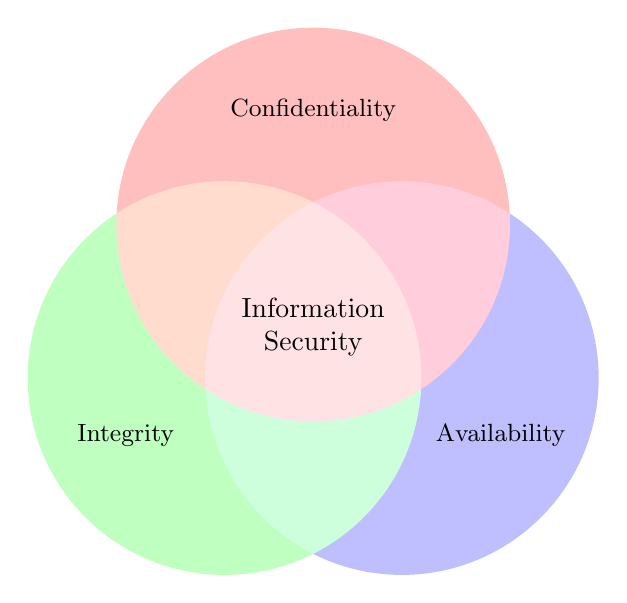
\begin{tikzpicture}
  \begin{scope}[blend group = soft light]
    \fill[red!25!white]   ( 90:1.3) circle (2.5);
    \fill[green!25!white] (210:1.3) circle (2.5);
    \fill[blue!25!white]  (330:1.3) circle (2.5);
  \end{scope}
  \node [font=\small] at (90:2.75)     {Confidentiality};
  \node [font=\small] at (210:2.75)    {Integrity};
  \node [font=\small] at (330:2.75)    {Availability};
  \node [align=center]			       {Information \\ Security};
\end{tikzpicture}
	\caption{The CIA information security triad.}
	\label{fig:cia}
\end{figure}
\pagebreak
\section{Content-Based Recommendation System}
In this section, we will examine each of the principal goals of the CIA triad in regards to content-based recommendation systems and explore various threats to these principles.
\subsection{Confidentiality}
The confidentiality of the data inside content-based recommendation systems is usually of relatively low significance since it contains no personal data, and all input data for the system, e.g., names, descriptions, categories, and images of items, are usually publicly available through the web service embedding the recommendation system. Therefore we see no unique risks regarding the confidentiality of content-based recommendation systems, and the common risks for web-services apply.
\subsection{Integrity}
Integrity, on the other hand, is essential to the successful deployment of any recommendation system. In the case of content-based recommendation systems, the integrity of predictions is mostly dependent on the quality of the input data, i.e., the item catalog. Figure~\ref{fig:attack-tree-content} summarizes the potential attacks on the integrity of this data, and the following paragraphs will explain each of the goals and attacks in detail.
\begin{figure}[H]
	\centering
	\begin{forest}
for tree={
  draw,
  align=center,
  l sep=1cm,
  s sep=0.25cm,
  anchor=north,
  child anchor=north,
  font=\small 
},
[{Manipulate the output \\ of a  content-based \\ recommendation system}, name=AD
  [{Decrease \\ overall performance}
  	[{Poison training\\ data with \\ mislabeled \\ items}]  
  ]
  [{Promote \\ target item}, and
  	[{Identify viable \\ attack item}]  
  	[{Maximize \\ similarity of \\ target item  \\ to attack item}]  
  ]
  [{Demote \\ target item}, and
  	[{Identify similar \\ items to target}]
  	[{Inject attack \\ items with \\ higher similarity \\ than target}]
  ]
]
\end{forest}
	\caption{Attack tree, summarizing the potential attacks on the integrity of content-based recommendation systems}
	\label{fig:attack-tree-content}
\end{figure}
\pagebreak
If the item catalog is accessible and editable by third parties, as in the case of marketplaces or social networks,  a defender needs to consider the risk of a malicious data injection. For example, an attacker trying to decrease the overall performance of such a system might try to inject mislabeled or corrupt items into the catalog to confuse the training algorithm and degrade the recommendation system's predictions, as seen in the leftmost leaves of the attack tree in Figure~\ref{fig:attack-tree-content}.

A more targeted attack could attempt to manipulate a target item aiming to maximize its similarity with other popular items to gain more views, as seen in the center of Figure~\ref{fig:attack-tree-content}. To perform such an attack, an adversary needs to know the type of algorithm and also has to have access to the contextual item data used by the algorithm to calculate item similarities. As previously mentioned, this data is usually easily acquirable through the crawling of publicly available web sites. Knowledge about the employed algorithm should also be considered publicly accessible as system security should not depend on the secrecy of the implementation or its components~\parencite{scarfone2008guide}.

Similar to the previous attack goal, an adversary could also attempt to demote a specific target item, as depicted in the right portion of Figure~\ref{fig:attack-tree-content}. In other words, to push it down in the list of recommended articles. We assume that the adversary has no control over the target item in this scenario as it could, for example, be under the control of a competitor. Since the adversary cannot manipulate the target item directly, the only way to demote the target item is to steal its recommendation slots. As the similarity measures used in content-based recommendations are usually symmetrical, the adversary might look at the target's recommendation results to determine its current recommendation slots. After identifying the items on which the target appears as a recommendation, the adversary could inject a set of attack items with a higher similarity than the target item to push it down the list of recommendations and steal its display space.
\subsection{Availability}
As the principal goals of availability and integrity are closely related, similar adversarial goals and risks arise. For example, an adversary trying to increase the overall error rate of the recommendation system will also violate availability at a certain point. Additionally, the universal availability risks for web-services, like a \ac{DDoS}, apply as well and should be considered in a complete threat model.

